\documentclass{article}
\usepackage{graphicx}
\usepackage{caption}
\usepackage{subcaption}
\usepackage{pgfplots}
\usepackage{blindtext}
\usepackage{multicol}
\usepackage{mathtools}
\usepackage{booktabs}
\usepackage[a4paper, total={6in, 9in}]{geometry}
\pgfplotsset{compat=1.18}
\usetikzlibrary{3d,calc}
\usepgfplotslibrary{groupplots}

\title{Discovering Artificial Neural Networks with Perceptrons}
\author{Ludovic DEBEVER}
\date{May 2024}

\begin{document}

\maketitle

\begin{figure}[!h]
    \centering
    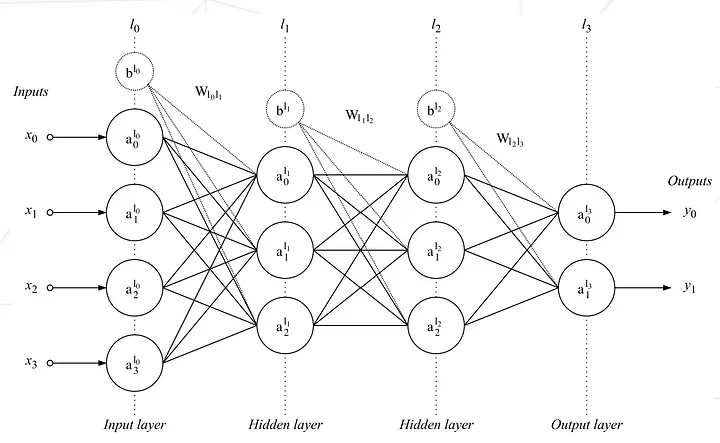
\includegraphics[width=1\linewidth]{assets/cover.png}
    \label{fig:cover}
\end{figure}

\newpage

\section{Introduction}

Artificial Intelligence (AI) is revolutionizing numerous fields, and healthcare is no exception. One of the most promising applications of AI in medicine is its use in assisting doctors to detect pneumonia through the analysis of chest X-rays. By leveraging advanced machine learning algorithms, AI systems can rapidly and accurately identify signs of pneumonia, often outperforming traditional methods. This technological breakthrough not only enhances diagnostic accuracy but also expedites treatment, ultimately improving patient outcomes. In this article, we explore how AI is transforming pneumonia detection, the technology behind it, and its implications for the future of medical diagnostics.

\begin{figure}[!htb]
\minipage{0.32\textwidth}
  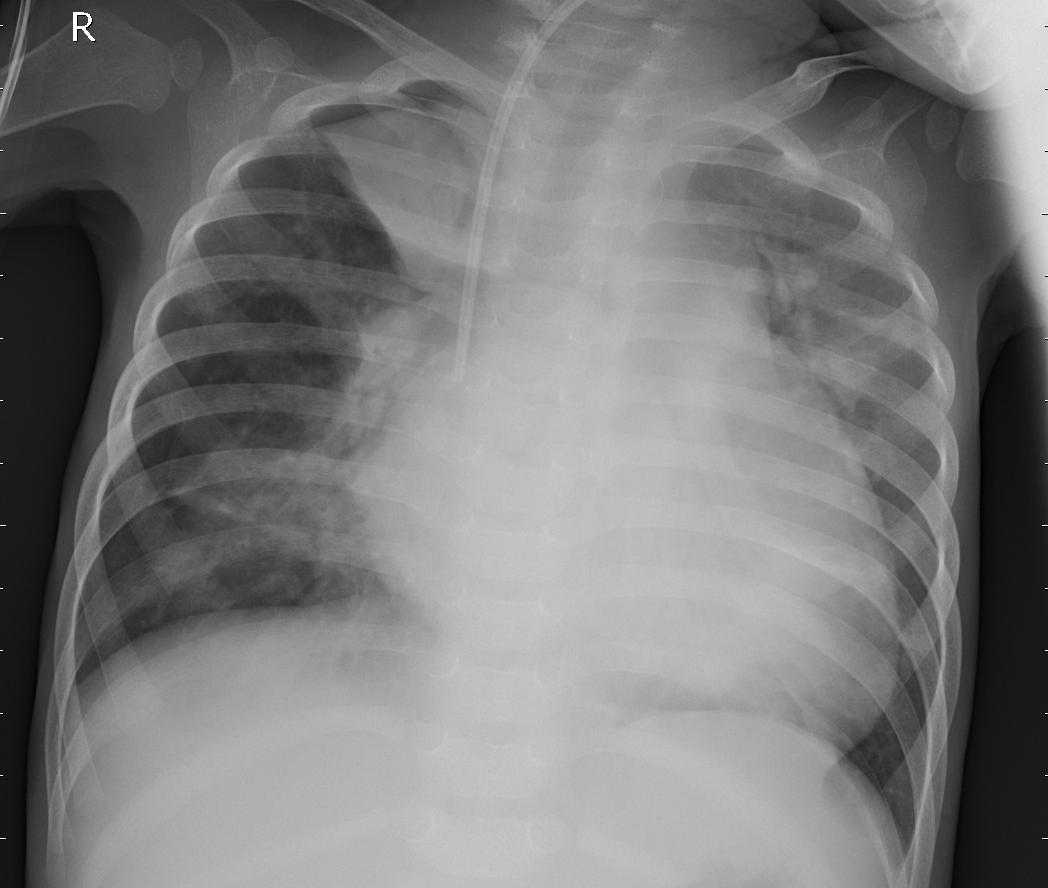
\includegraphics[width=\linewidth]{assets/intro/scan-bacteria.jpeg}
  \caption*{Bacteria}\label{fig:scan-bacteria}
\endminipage\hfill
\minipage{0.32\textwidth}
  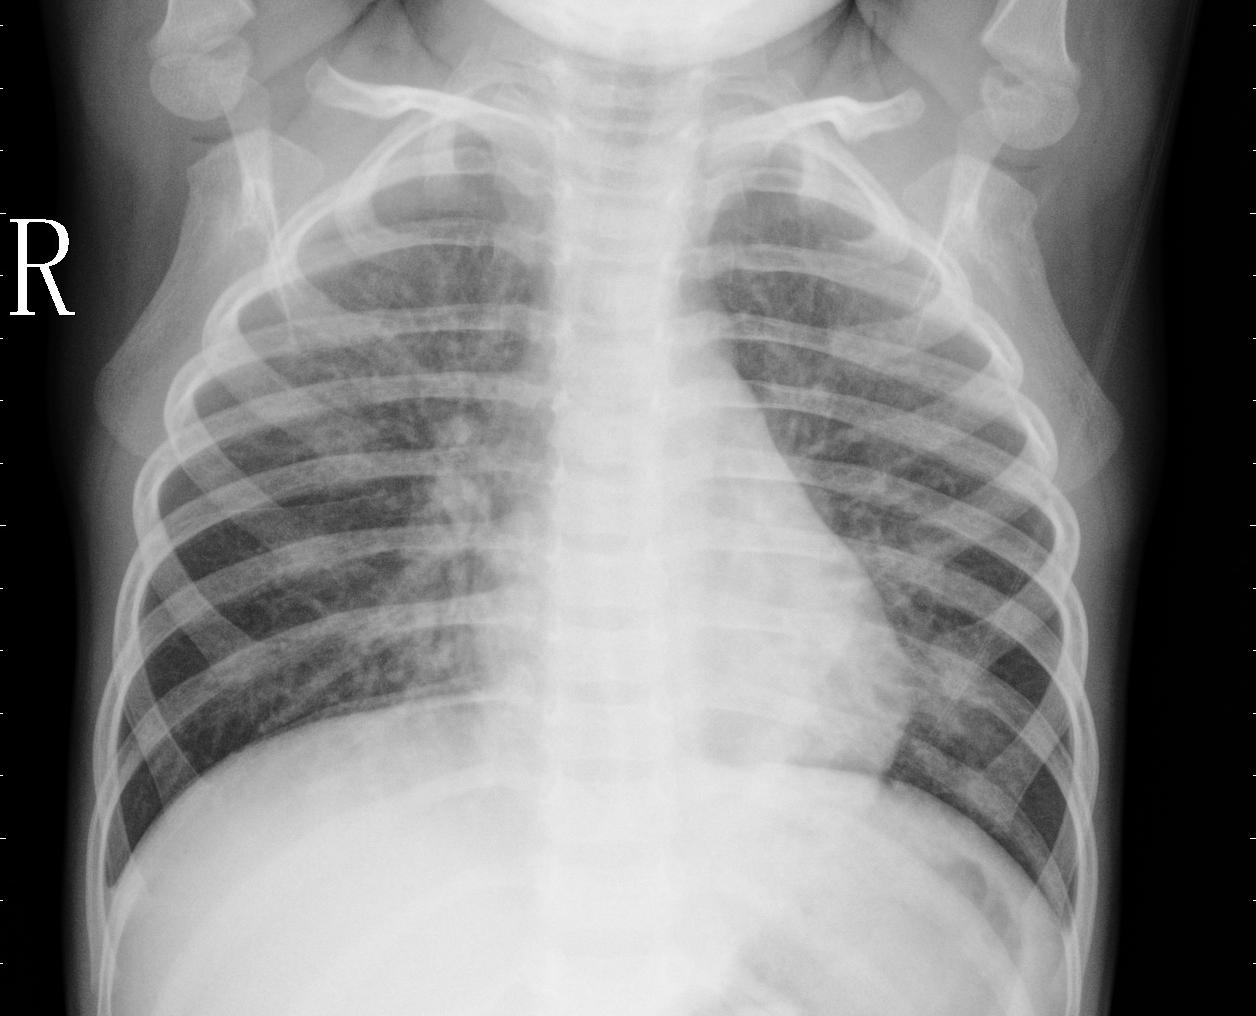
\includegraphics[width=\linewidth]{assets/intro/scan-virus.jpeg}
  \caption*{Virus}\label{fig:scan-virus}
\endminipage\hfill
\minipage{0.32\textwidth}%
  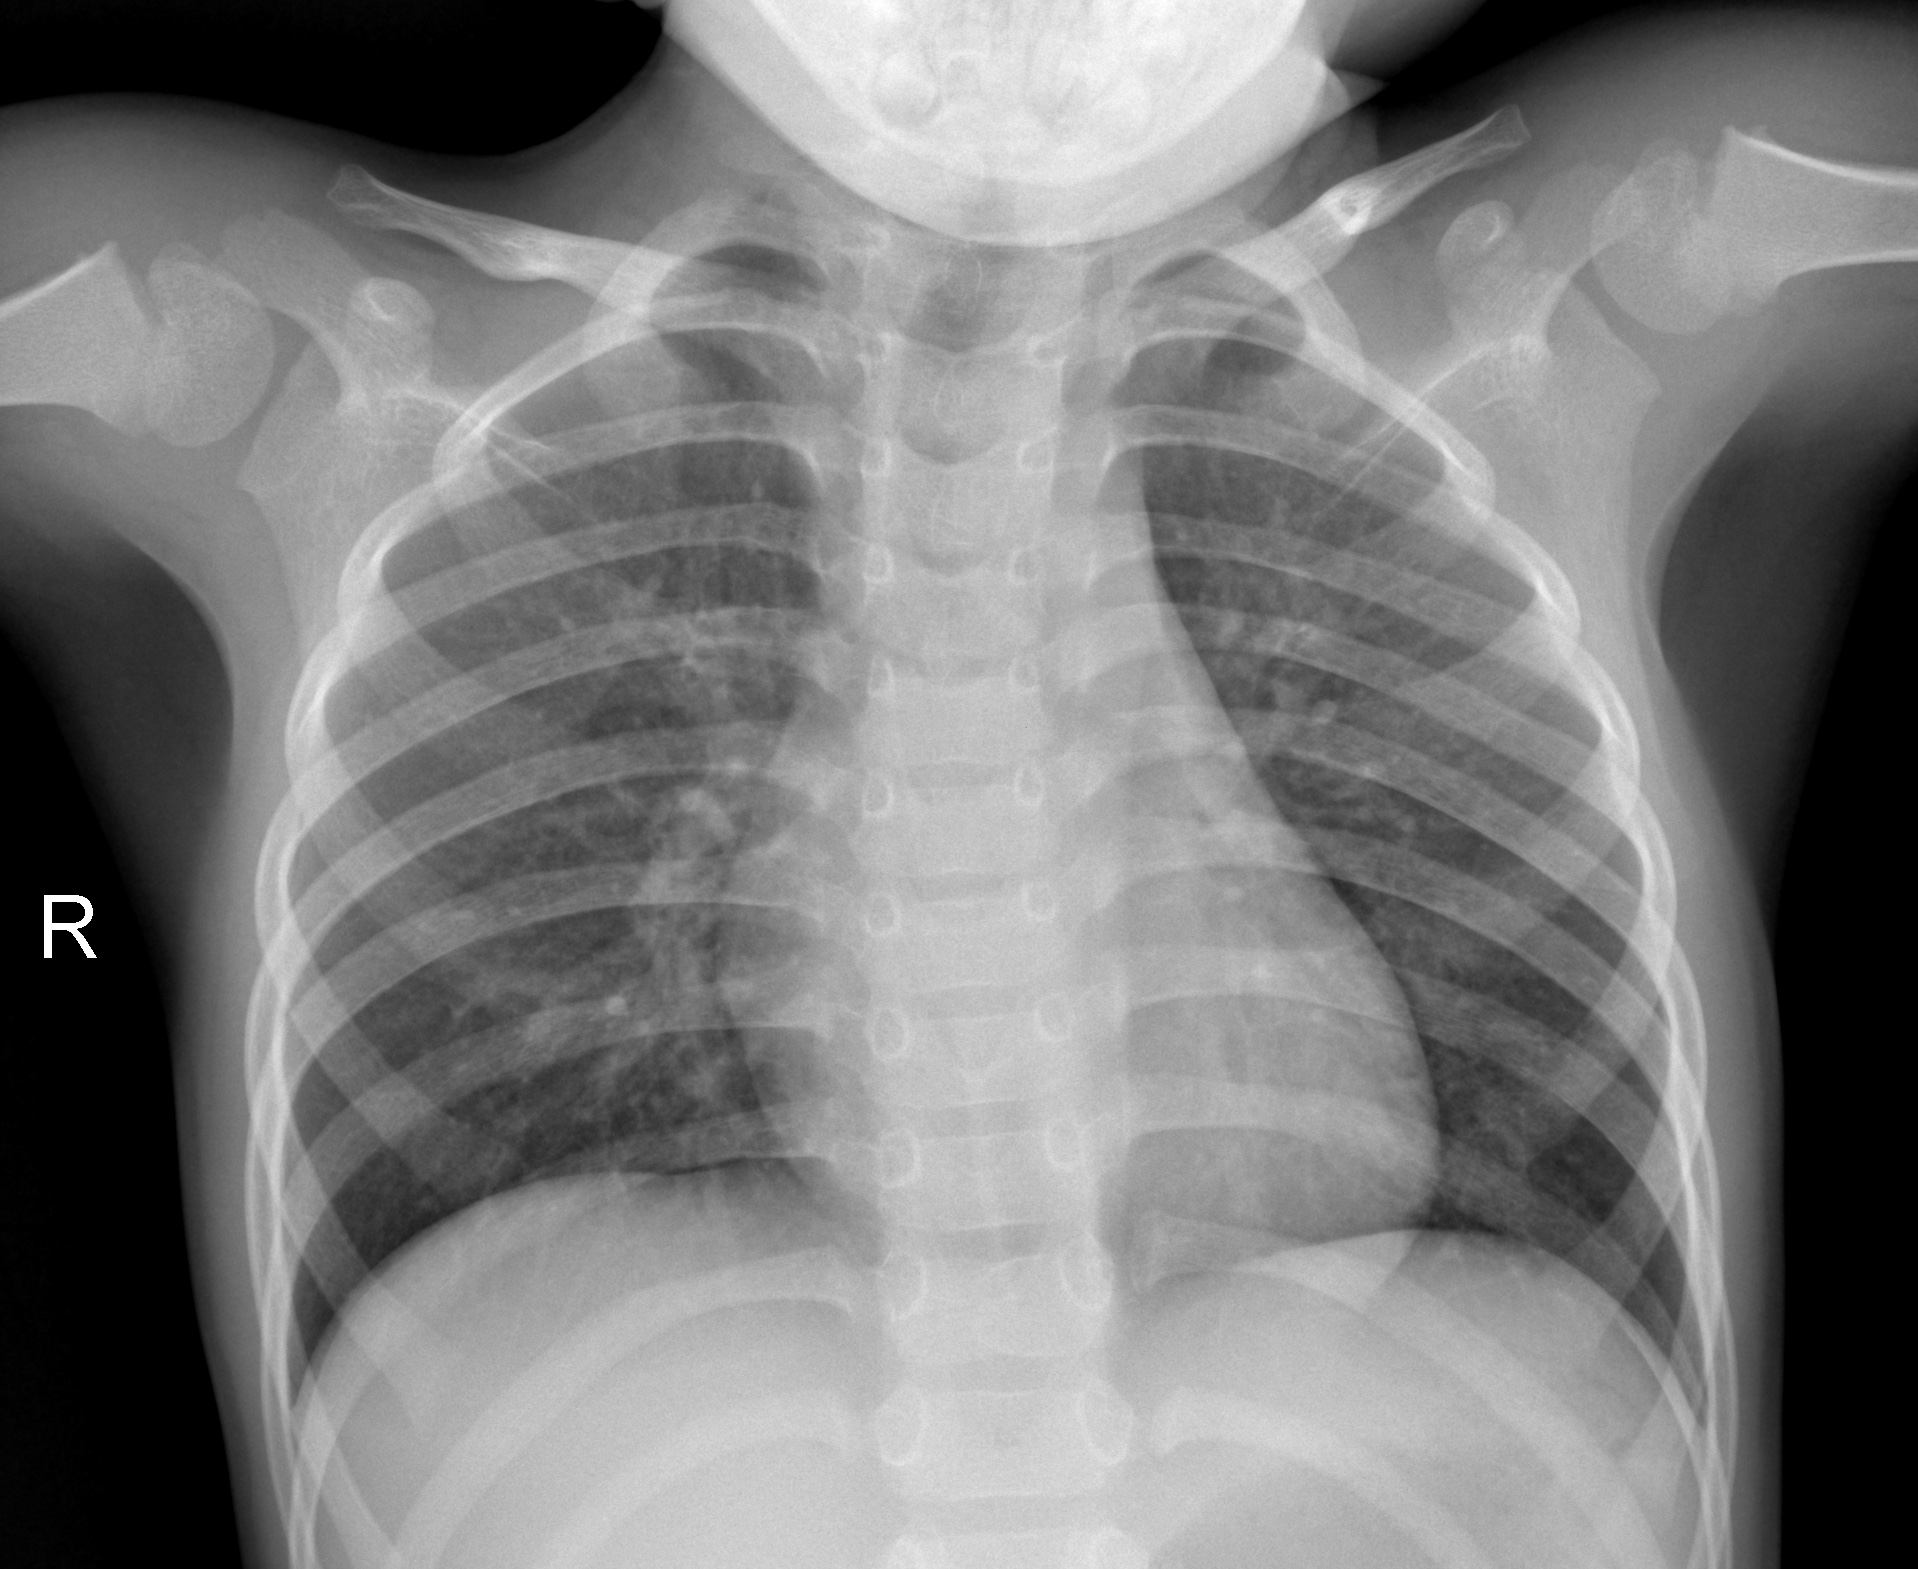
\includegraphics[width=\linewidth]{assets/intro/scan-normal.jpeg}
  \caption*{Normal}\label{fig:scan-normal}
\endminipage
\end{figure}

\section{Frank Rosenblatt's Perceptron}

In 1957, Frank Rosenblatt invented the Perceptron, the simplest form of neural network and one of the first models to demonstrate machine learning. This groundbreaking model laid the foundation for future advancements in the field, as it was one of the earliest systems capable of learning from data. A model that would later be applied to fields such as image processing and speech recognition, it showcased the potential of machine learning to tackle complex tasks by improving performance through experience.

Based on a simple algorithm, the Perceptron could adapt to the input data in order to perform better over time. However, despite its innovative approach, the Perceptron had hard limitations. It could not solve non-linear problems, meaning it struggled with tasks where the relationship between input and output was not straightforward. This limitation was famously highlighted by Marvin Minsky and Seymour Papert in their 1969 book "Perceptrons," which demonstrated that the Perceptron could not handle the XOR problem, a simple example of a non-linear classification task.

\newpage

\subsection{How does a Perceptron learn?}

The Perceptron involves principles that are foundational to modern artificial intelligence. It comprises key components such as Inputs and Weights, an Activation Function, and Back-propagation. At its core, the Perceptron is a single neuron directly connected to the inputs. Each input is assigned a specific weight, which represents its importance in the prediction process. To make a prediction, the Perceptron calculates the weighted sum of all inputs, which is the sum of each input multiplied by its corresponding weight.

Once the weighted sum is computed, the Perceptron employs an activation function to determine the output. In this simplified model, we use a threshold as the activation function. If the weighted sum exceeds the set threshold, the Perceptron produces a positive result; otherwise, it returns a negative result. This binary classification process allows the Perceptron to distinguish between two classes based on the input data.

\begin{figure}[ht]
    \caption*{Perceptron}
    \centering
    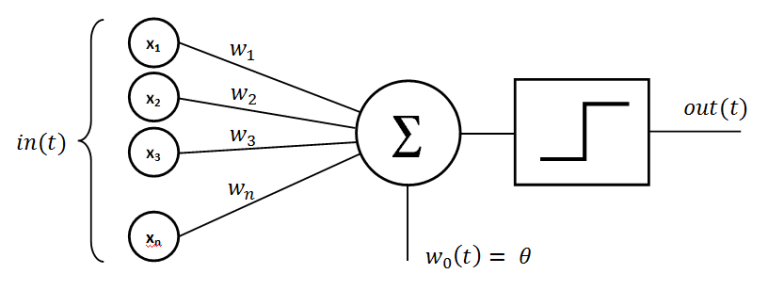
\includegraphics[width=0.75\linewidth]{assets/perceptron/perceptron.png}
    \label{fig:perceptron}
\end{figure}
To improve its performance over time, the Perceptron uses a learning process called Back-propagation. During training, the Perceptron adjusts its weights based on the errors between the predicted and actual outcomes. By iteratively updating the weights to minimize these errors, it learns to make more accurate predictions. 

In some rare cases we may encounter a set of inputs that sum to 0, with such input, no matter the weights the result will always be 0. To avoid this issue we use a concept called bias. It is a complementary input that we add with a fixed value of 1, so that no matter the input, the result can always be different than 0.

\begin{figure}[ht]
    \caption*{Perceptron with bias}
    \centering
    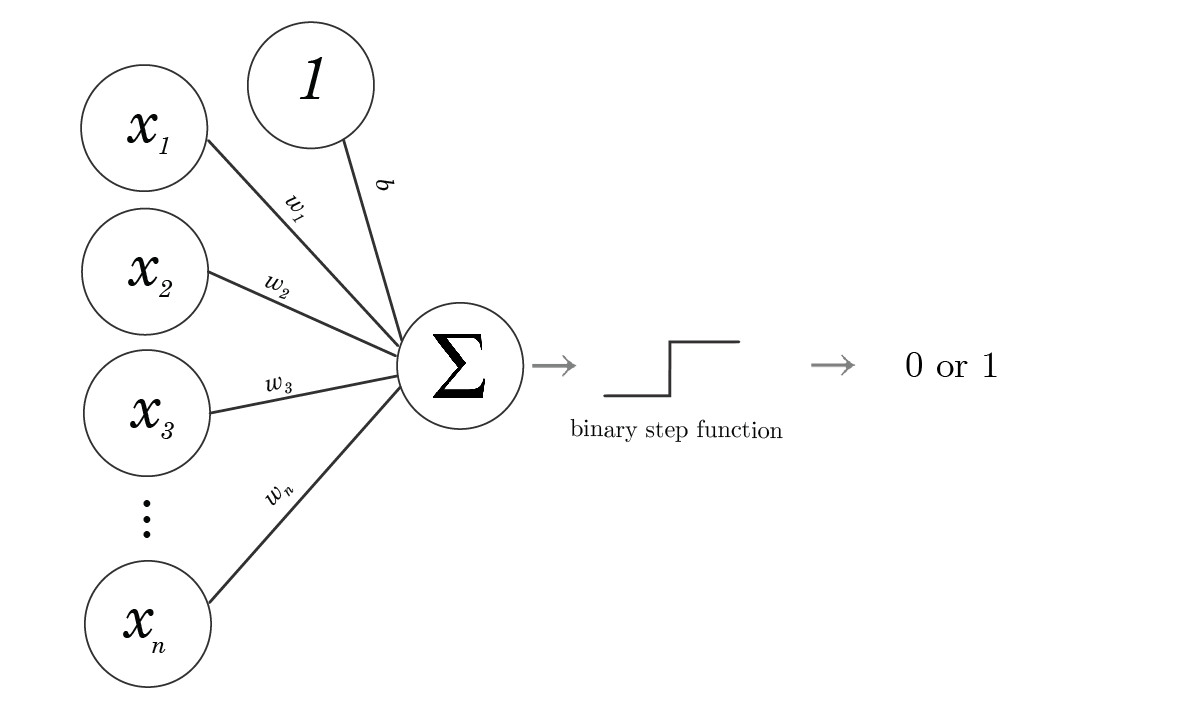
\includegraphics[width=0.75\linewidth]{assets/perceptron/perceptron-bias.png}
    \label{fig:perceptron-bias}
\end{figure}

\newpage

\subsection{Classifying Images using the Perceptron}

Using this model, we can classify images. However, due to the Boolean nature of the Perceptron's output, it can only differentiate between two classes, which is enough in our case. Before we proceed, we need to normalize our data. Each image will be resized to a fixed number of pixels—64x64 in this case—which provides a good balance between detail and low memory usage. Then, the color ranges will be converted to gray-scale values, leaving us with a single number per pixel. Each of these gray-scale values will serve as an input to the Perceptron.

\begin{figure}[ht]
    \centering
    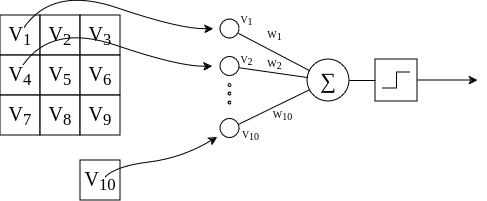
\includegraphics[width=0.75\linewidth]{assets/perceptron/perceptron-image-classification.png}
    \caption*{Image Classification Perceptron}
    \label{fig:perceptron-image-classification}
\end{figure}

The final step before starting the training process is to define the hyper-parameters, which are the human-controlled settings of the model. For a Perceptron, these include the learning rate, the activation function, the number of epochs, and the number of inputs. We will use a simple threshold for the activation function, and the number of inputs has already been established during data normalization. Therefore, we only need to define the learning rate and the number of epochs. The learning rate is crucial during the Perceptron's learning phase; after predicting a value and calculating the error, the error is multiplied by the learning rate and used to adjust the weights accordingly. The learning rate needs to be small enough to allow the back-propagation process to find precise values for the Perceptron's weights. 

Finally, the number of epochs define how many times the training process will go through the entire dataset. Perceptrons cannot be over-fit and are very quick to train due to its simple structure, so setting a high number of epochs should not disturb the training process.

Due to the simple structure of the Perceptron, visualizing its weights is quite simple. By assigning one weight per pixel, we can generate an image that mirrors the properties of our normalized training data, providing a glimpse into the Perceptron's "brain." Additionally, when predicting an image, we can combine each pixel's value with the corresponding weight from the Perceptron and normalize the result. This allows us to see what the Perceptron focuses on during image prediction.

\begin{figure}[!ht]
\centering
\caption*{Weights of the Perceptron after 25 epochs on a single prediction.}
\begin{subfigure}{0.25\textwidth}
  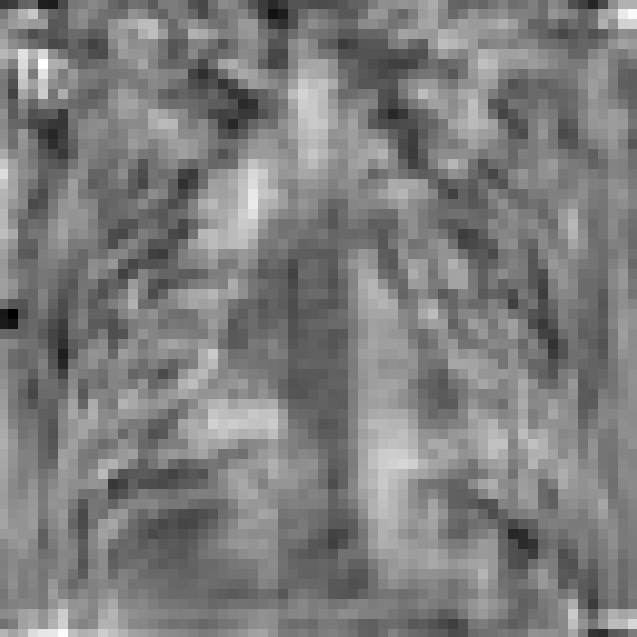
\includegraphics[width=\linewidth]{assets/perceptron/training-1-weights.png}
  \caption*{Weights}\label{fig:training-1-weights}
\end{subfigure}
\xspace
\begin{subfigure}{0.25\textwidth}
  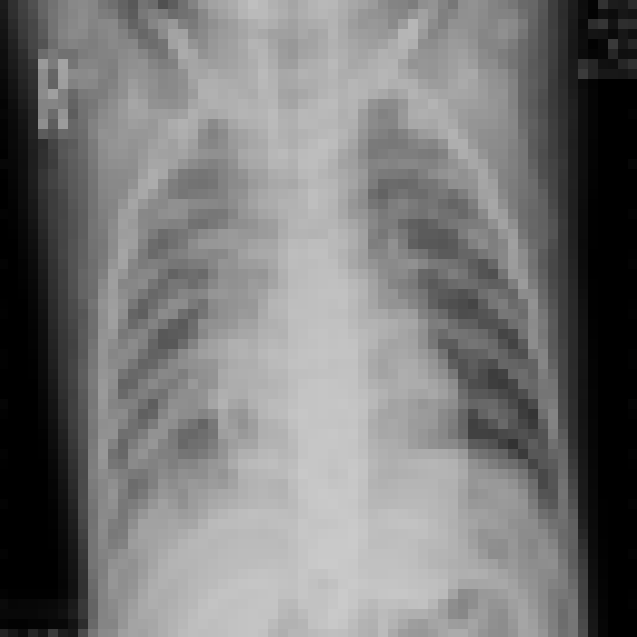
\includegraphics[width=\linewidth]{assets/perceptron/training-1-predict.png}
  \caption*{Predicted}\label{fig:training-1-predicted}
\end{subfigure}
\xspace
\begin{subfigure}{0.25\textwidth}%
  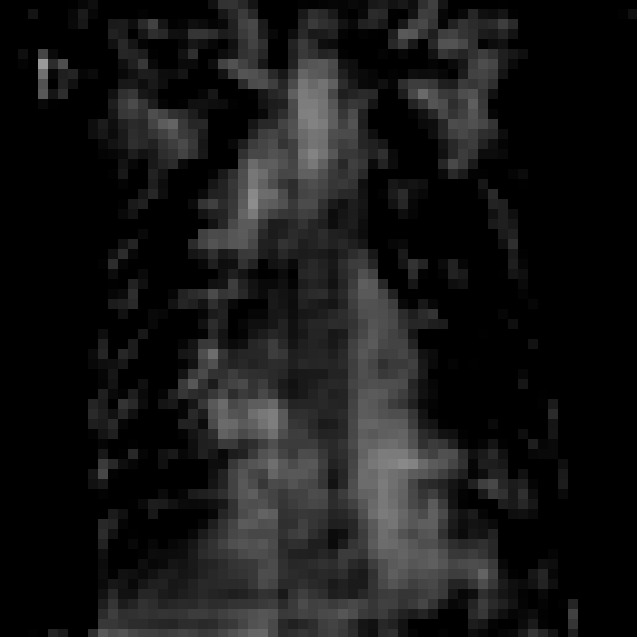
\includegraphics[width=\linewidth]{assets/perceptron/training-1-add.png}
  \caption*{Weights + Predicted}\label{fig:train-1-subtract}
\end{subfigure}
\end{figure}
\newpage

\begin{figure}[!ht]
\centering
\caption*{Evolution of weights over epochs}
\begin{subfigure}{0.22\textwidth}
  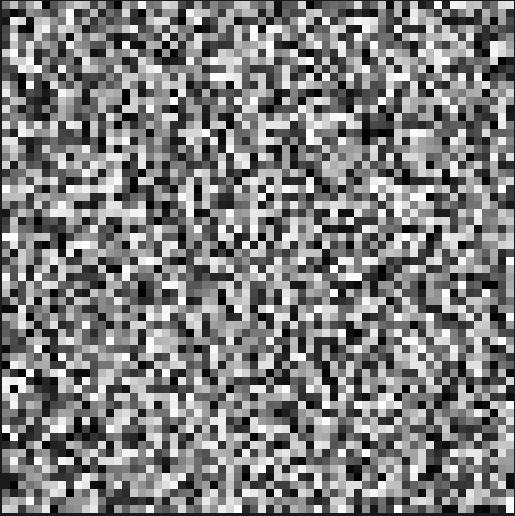
\includegraphics[width=\linewidth]{assets/perceptron/training-1-epoch-0.png}
  \caption*{Epoch 0}\label{fig:training-1-epoch-0}
\end{subfigure}
\xspace
\begin{subfigure}{0.22\textwidth}
  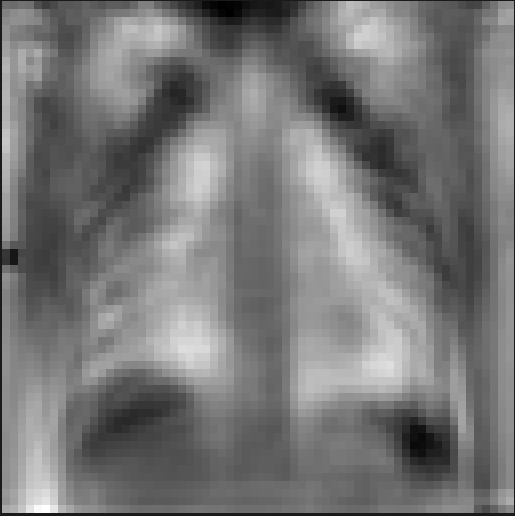
\includegraphics[width=\linewidth]{assets/perceptron/training-1-epoch-1.png}
  \caption*{Epoch 1}\label{fig:training-1-epoch-1}
\end{subfigure}
\xspace
\begin{subfigure}{0.22\textwidth}%
  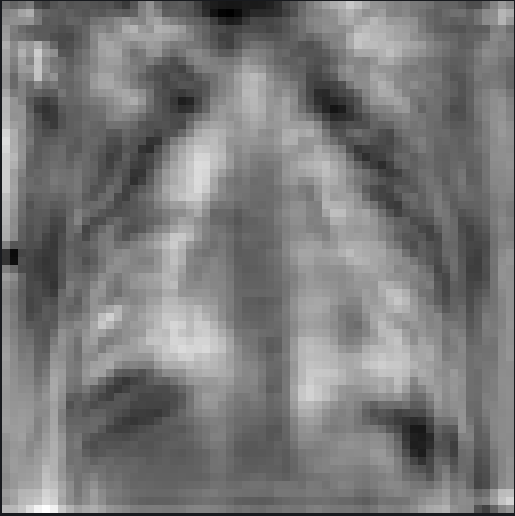
\includegraphics[width=\linewidth]{assets/perceptron/training-1-epoch-4.png}
  \caption*{Epoch 4}\label{fig:train-1-epoch-4}
\end{subfigure}
\xspace
\begin{subfigure}{0.22\textwidth}%
  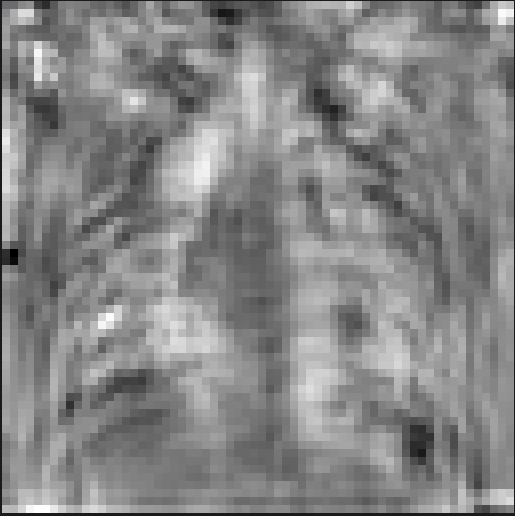
\includegraphics[width=\linewidth]{assets/perceptron/training-1-epoch-16.png}
  \caption*{Epoch 16}\label{fig:train-1-epoch-16}
\end{subfigure}
\end{figure}

\begin{multicols}{2}

When analyzing the accuracy trend over multiple epochs in training a Perceptron, a significant fluctuation often indicates that the model is struggling to find an optimal solution. This issue is frequently caused by an excessively high learning rate, which results in back-propagation overshooting while trying to adjust the weights based on the error. Essentially, the adjustments made during training are too large, causing the model to oscillate around the optimal point rather than converging to it.

\begin{tikzpicture}[font=\scriptsize]
    \begin{axis}[
        width=\linewidth,
        axis line style={draw=none},
        xlabel=Epoch,
        ylabel=Accuracy (\%)
    ]
        \addplot[teal] table [x=Epoch,y=Accuracy]{assets/perceptron/training-1.txt};
    \end{axis}
\end{tikzpicture}

To mitigate this problem, implementing a learning rate scheduler can be beneficial. A learning rate scheduler dynamically adjusts the learning rate during training, typically decreasing it as the training progresses to allow for finer adjustments. There are several types of learning rate schedulers, but in this case, three specific types were tested: Step Decay, Exponential Decay, and Cosine Annealing.

Step Decay reduces the learning rate by a factor at specified intervals. Exponential Decay continuously decreases the learning rate exponentially. Cosine Annealing, on the other hand, adjusts the learning rate following a cosine function.

In practice, Step Decay has shown the most positive impact on accuracy among the tested methods. This approach allows the learning rate to be lowered in a controlled, step-wise manner, which seems to aid the model in converging more effectively by balancing between fast initial learning and stable final adjustments.

\begin{tikzpicture}[font=\scriptsize]
    \begin{axis}[
        width=\linewidth,
        axis line style={draw=none},
        xlabel=Epoch,
        ylabel=Accuracy (\%)
    ]
        \addplot[teal] table [
                mark=none,
                x=Epoch,
                y=Accuracy
            ]{assets/perceptron/training-2.txt};
    \end{axis}
\end{tikzpicture}

\end{multicols}

\newpage

\section{The XOR Problem}
    
The XOR Problem is a simple non-linear problem that shows the limitations of Perceptrons. First let's talk about the AND and OR operations. These are logical operations that takes two inputs in the form of a boolean value and produce a single output. AND simply returns 1 when both inputs are 1, otherwise it will return 0. OR, returns 1 of one of the inputs is 1, otherwise 0. Finally, XOR will return 1 if both inputs are different.

When displaying these operators outputs in a table such that columns are input A and rows are input B, We can easily separate the ones from the zeros in a single straight line for AND and OR. But when trying to do the same with XOR, the problem becomes apparent. We need two lines.

\section{Multi Layer Perceptrons}

In order to make neural networks able to solve non-linear problems, we can use what is called a Multi Layer Perceptron. It is a succession of Perceptrons organized into layers of different type: 

\begin{itemize}
    \item The Input Layer, which is just the same as with a regular Perceptron.
    \item The Output Layer, this is the last layer, where we get the result from.
    \item The Hidden Layer(s), are every layers between the input, and the output layers.
\end{itemize}

\begin{figure}[!h]
    \centering
    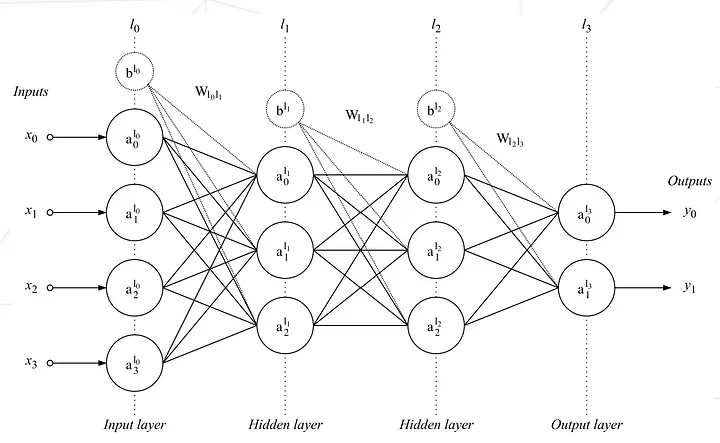
\includegraphics[width=.75\linewidth]{assets/cover.png}
    \label{fig:multi-layer-perceptrons}
\end{figure}

\end{document}


% caption under the images
% table cpation over